%% IMPORTANT: Once working, run latex 3 times to get listoffigures to work

%% Be sure to check spelling!

%% Put your name and the proper due date in place

%% Copy the lstinputlisting and figure code as many times as you need
%% Be sure to put in your own file names if appropriate

%% Note that the \epsfig and \lstinputlisting commands 
%% are currently commented out with %%% - until the
%% files exist, processing this code without them will result in an error
%% so leave the comments until you have created the files!

%%% Items starting with %%% are actionable items

\documentclass{article}
\usepackage{amsmath}    % loads AMS-Math package
\usepackage{epsfig}     % allows PostScript files
\usepackage{listings}   % allows lstlisting environment
\usepackage{moreverb}   % allows listinginput environment
\usepackage[letterpaper, margin=0.75in]{geometry}  % set paper size/margins
\usepackage{EGR103F19}  % colorful file imports

\begin{document}
\begin{center}
\rule{6.5in}{0.5mm}\\~\\
\textbf{\large EGR 103L -- Fall 2019}\\~\\
\textbf{\huge Laboratory 8 - Surfaces}\\~\\
Marcus Deansd (md374)\\
Lab Section 4, Tuesdays 11:45-2:35\\
17 November 2019\\~\\
{\small I understand and have adhered to all the tenets of the Duke
  Community Standard in completing every part of this assignment.  I
  understand that a violation of any part of the Standard on any part
  of this assignment can result in failure of this assignment, failure
  of this course, and/or suspension from Duke University.} 
\rule{6.5in}{0.5mm}\\
\end{center}
\tableofcontents
\listoffigures
\renewcommand{\arraystretch}{1.5}
\clearpage

\section{Chapra 2.22}
The graph is smoother at the beginning of both curves with comparison to the end. This is due to the spacing of the data points (originating in the initial domain function). At the start, these data points are more dense and thus when the 'dots' of the data points are connected, they are so close together so as to appear as a smooth line. Near the end of both curves, the size of the  curve is larger so the distance is increasing while the number of data points remains constant, so the density goes down for that interval. This lower density means that the 'dots' of the data points, when connected, create a perceptibly non-smooth line as they are too far apart. This problem would be rectified by increasing the number of points in the domain, either in general or over that specific area of the domain. 

\section{Chapra 3.9}
This graph demonstrates that the velocity increases when either heigh of width increases, or both. There is direct relationship between them. An increase in width for a fixed height seems to more significantly increase the velocity compared to an increase in height for a fixed width; this was determined due to the increased number of striated colour bands on the right side of the graph (corresponding to changes in height) compared to the left side of the graph (corresponding to change in width). Each comparison was made while holding the other type constant. Regardless, both were found to have significant effect on velocity with the velocity being maximized when both height and width were at their maximum values. Furthermore, it was observed that \textbf{both} affected velocity to a large extent, as opposed to one factor having a large effect and the other not corresponding to significant change in velocity. This overall makes sense considering the equation used to obtain this result (specifically the roots).

\section{Chapra 15.5}
Strong relationships were observed between the temperature and chlorie concentration and the oxygen concentration. Namely, for any given temperature, the oxygen concentration decreased as chloride concentration went up. Therefore, the chloride concentration has an inverse relationship with oxygen concentration. Temperature was also found to have an inverse relationship with chloride concentration. As the temperature decreased for a given chloride concentration, the oxygen concentration rapidly increased. Therefore, the maximum oxygen concentration would be found at a temperature and chloride concentration of 0, while the lowest oxygen concentration would result from the greatest chloride concentration and temperature ($20 g/L$ and $30$ Celsius, respectively). 

\section{Chapra 15.6}
Using a planar model:
\begin{align*}
\hat{OC}(c, T)&=\sum_ma_m\phi_m(c,T)=a_0(c^0T^0)+a_1(c^1)+a_2(T^1)
\end{align*}
the model coefficients and other required values are:
\begin{center}
\begin{tabular}{c|c|c|c|c|c}
$a_0$ & $a_1$ & $a_2$ & $r^2$ & $OC(15, 12)$ g/ml & $\epsilon_t$ \\ \hline
 13.52 & -0.1049 &  -0.2012& 9.659e-01& 9.533 &  4.88\%
\end{tabular}
\end{center}
% discussion
The graph of the residuals could most likely be modeled effectively using equations for parabolas. With the graph roughly forming the shape of a 'U' with its peaks, parabolas could be used to approximate this to various extents depending on the region. In terms of trends, the residuals were highest when the chloride concentration and temperature were lowest (around 0 in particular) and when the chloride concentration and temperature were highest (specifically near 30). This two regions serve as key areas of examination in order to produce equations that could accurately model this. 

\section{Chapra 15.7}
Using a first-order model for $c$ and a third-order model for $T$:
\begin{align*}
\hat{OC}(c, T)&=
\sum_ma_m\phi_m(c, T)=a_0(c^0T^0)+a_1(c^1)+a_2(T^3)+a_3(T^2)+a_4(T^1) 
\end{align*}
the model coefficients and other required values are:
\begin{center}s
\begin{tabular}{c|c|c|c|c|c|c|c}
$a_0$ & $a_1$ & $a_2$ & $a_3$ & $a_4$ & $r^2$ & $OC(15, 12)$ g/ml & $\epsilon_t$ \\ \hline
1.403e01 & -1.049e-1 & -4.370 & 5.744e-03 & -3.364e-01 & 9.877e-01  & 9.168 & 0.856\%
\end{tabular}
\end{center}
% discussion
At first glance, the residuals seemed difficult to model using simple, common equations. With the directionality of the peaks and lows of the residuals, it seemed much more complex than the prior situation. The trend of higher residuals with maximums for chloride concentration and temperature, and minimums, held true. These areas still had high residuals. However, the residuals were dramatically reduced in the areas where the two factors were moving inversely of one another - when chloride concentration was high but temperature was low, and vice versa, the residuals were minimized in this model. Again, developing an accurate model would be difficult. Based on online research, it seemes that a hyperbolic paraboloid would be the srtructure created by the equations to model this graph, which would allow both the minima and maxima of the residuals to be incorporated into the model.

\section{Sphere}
Transformation equations:
\begin{align*}
x&=\rho * sin(\phi)*cos(\theta)\\
y&=\rho * sin(\phi)*sin(\theta)\\
z&=\rho * cos(\phi)
\end{align*}
\pagebreak

\appendix
\section{Codes}
% Put the name of your file in the subsection name 
% and the lstinputlisting - note that _ need to be \_ in 
% subsection name but not in lstinpustlisting name!

% Be sure to include the community standard in codes!

% Add \pagebreaks if they make sense

% Set default to python
\lstset{style=python103, language=python} 

\subsection{Chapra 2.22}
\lstinputlisting{Chapra_2.22_.py}
\pagebreak

\subsection{Chapra 3.9}
\lstinputlisting{Chapra_3.9_.py}
\pagebreak

\subsection{Chapra 15.5}
\lstinputlisting{Chapra_15.5_.py}
\pagebreak

\subsection{Chapra 15.6}
\lstinputlisting{Chapra_15.6_.py}
\pagebreak

\subsection{Chapra 15.7}
\lstinputlisting{Chapra_15.7_.py}
\pagebreak

\subsection{Sphere}
\lstinputlisting{Sphere.py}

\clearpage % start Figures on new page

\section{Figures}
% Remove %%% when ready; use your file names if different from mine

\begin{figure}[ht!]
\begin{center}
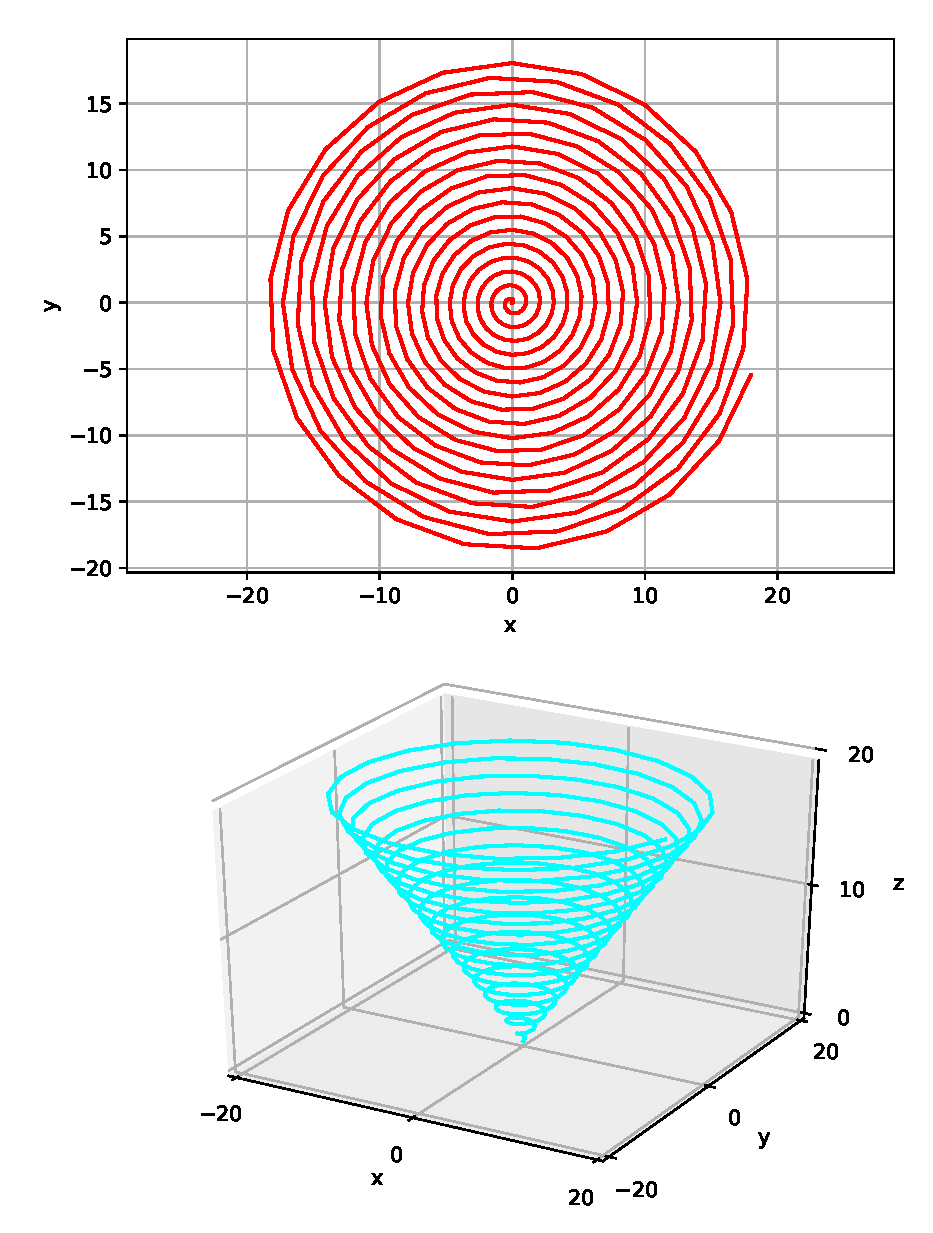
\epsfig{file=Chapra_2.22_Plot.eps}
\caption{Figure for Chapra 2.22}
\end{center}
\end{figure}

\begin{figure}[ht!]
\begin{center}
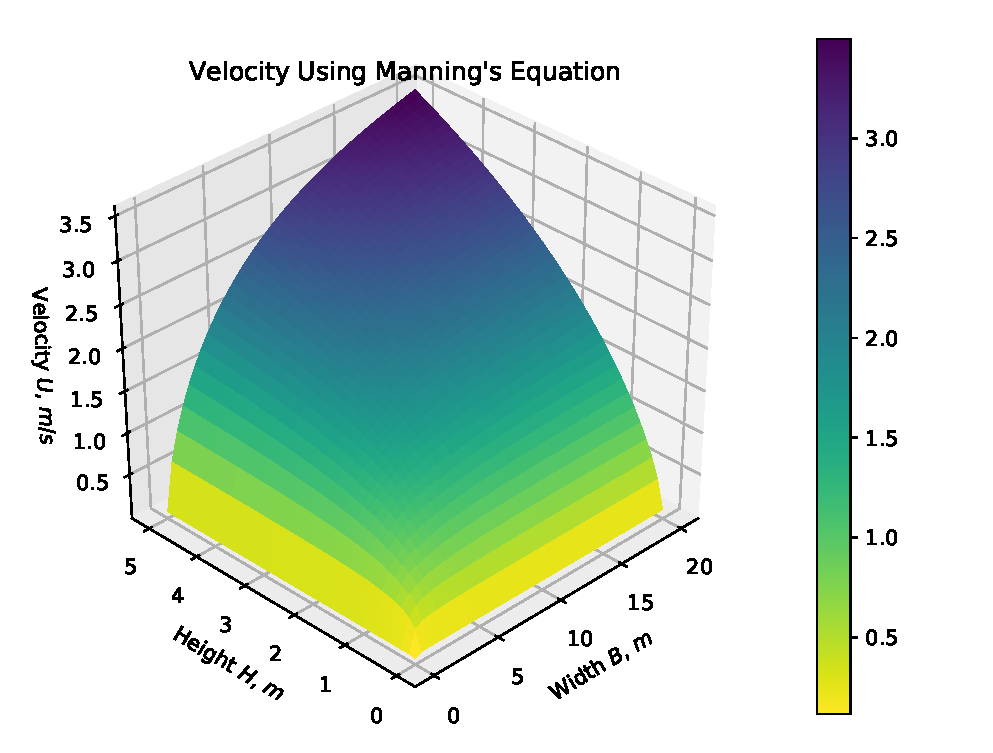
\epsfig{file=Chapra_3.9_Plot.eps}
\caption{Figure for Chapra 3.9}
\end{center}
\end{figure}

\begin{figure}[ht!]
\begin{center}
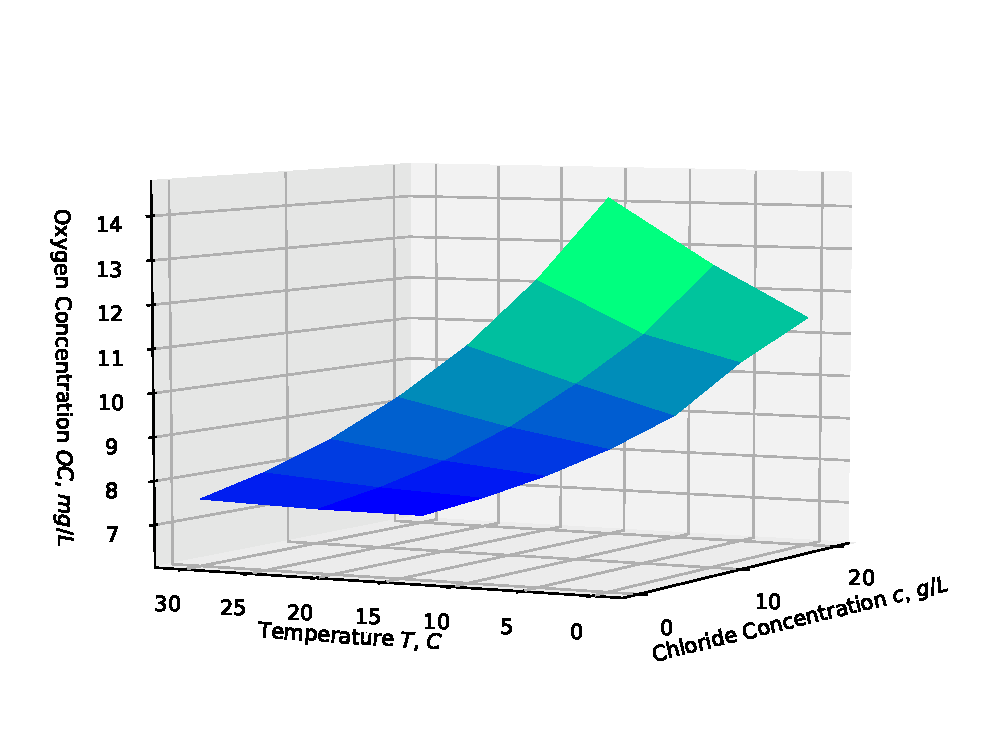
\epsfig{file=Chapra_15.5_Plot.eps}
\caption{Figure for Chapra 15.5}
\end{center}
\end{figure}

\begin{figure}[ht!]
\begin{center}
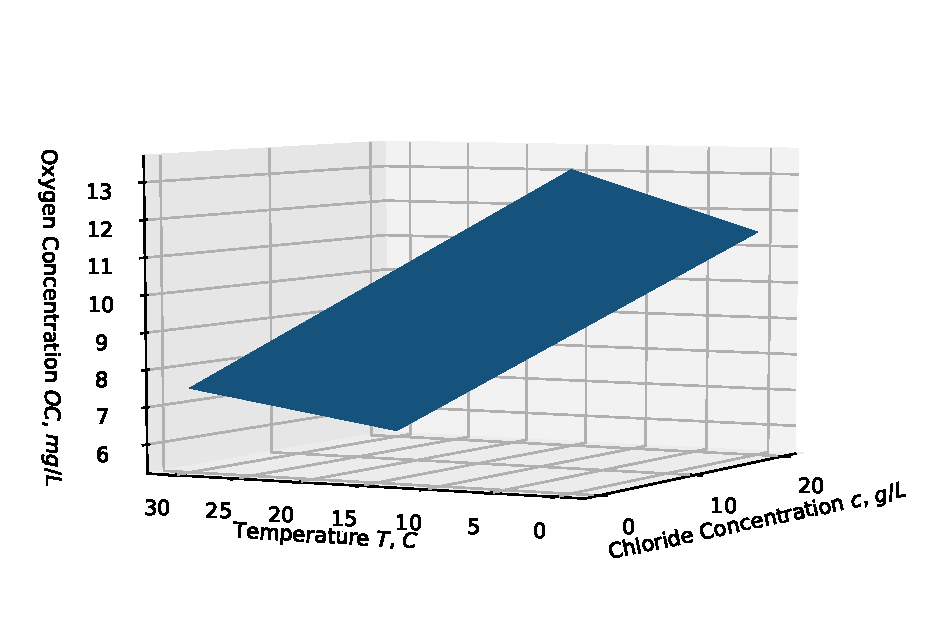
\epsfig{file=Chapra_15.6_Plot_Alpha.eps}\\
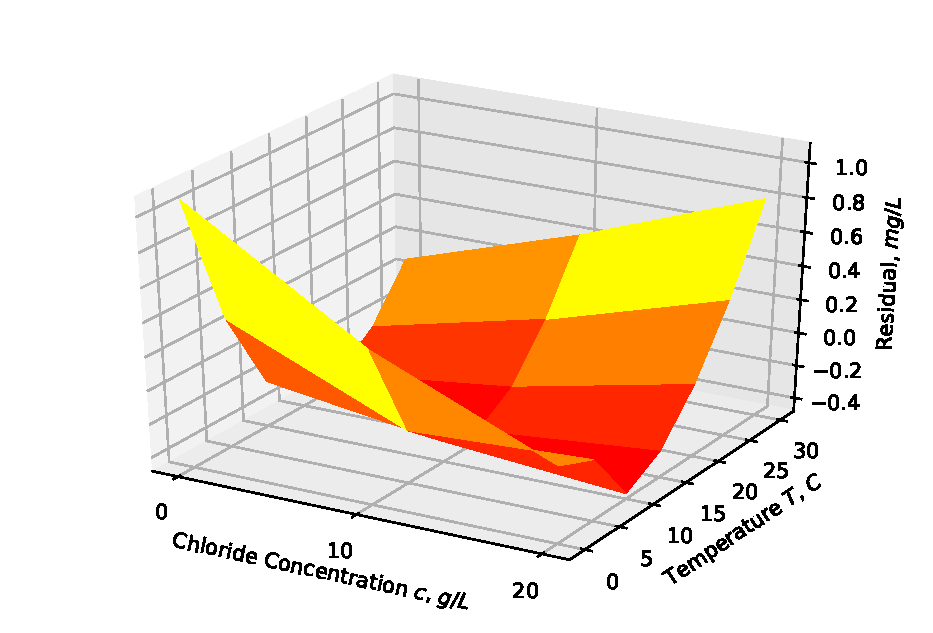
\epsfig{file=Chapra_15.6_Plot_Bravo.eps}
\caption{Figures for Chapra 15.6}
\end{center}
\end{figure}

\begin{figure}[ht!]
\begin{center}
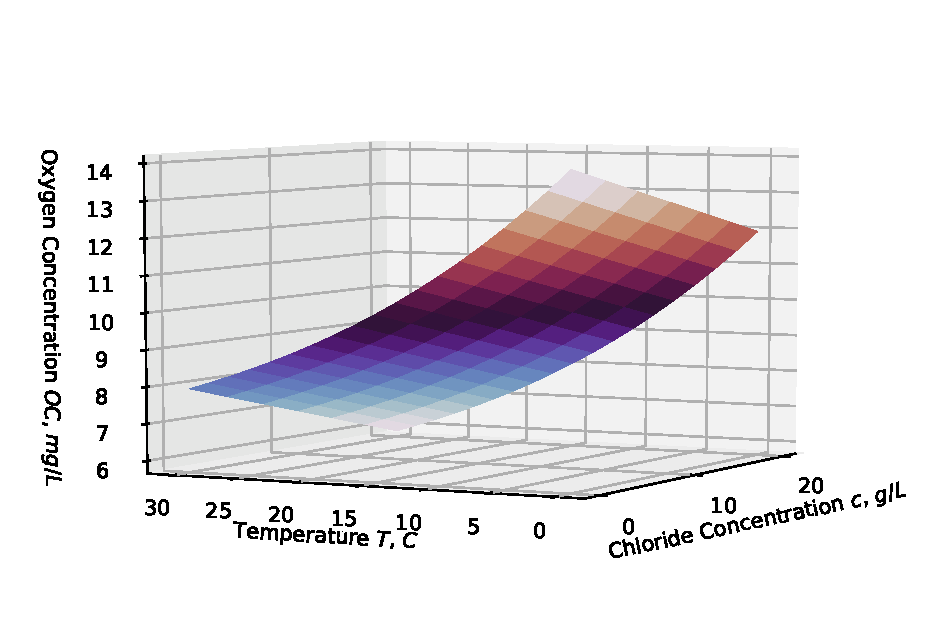
\epsfig{file=Chapra_15.7_Plot_Alpha.eps}\\
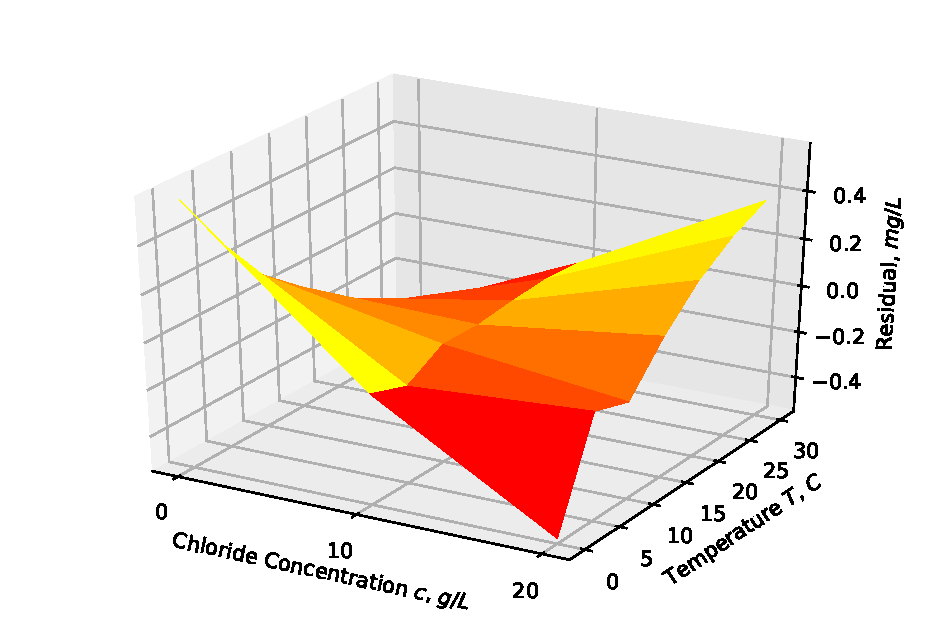
\epsfig{file=Chapra_15.7_Plot_Bravo.eps}
\caption{Figures for Chapra 15.7}
\end{center}
\end{figure}

\begin{figure}[ht!]
\begin{center}
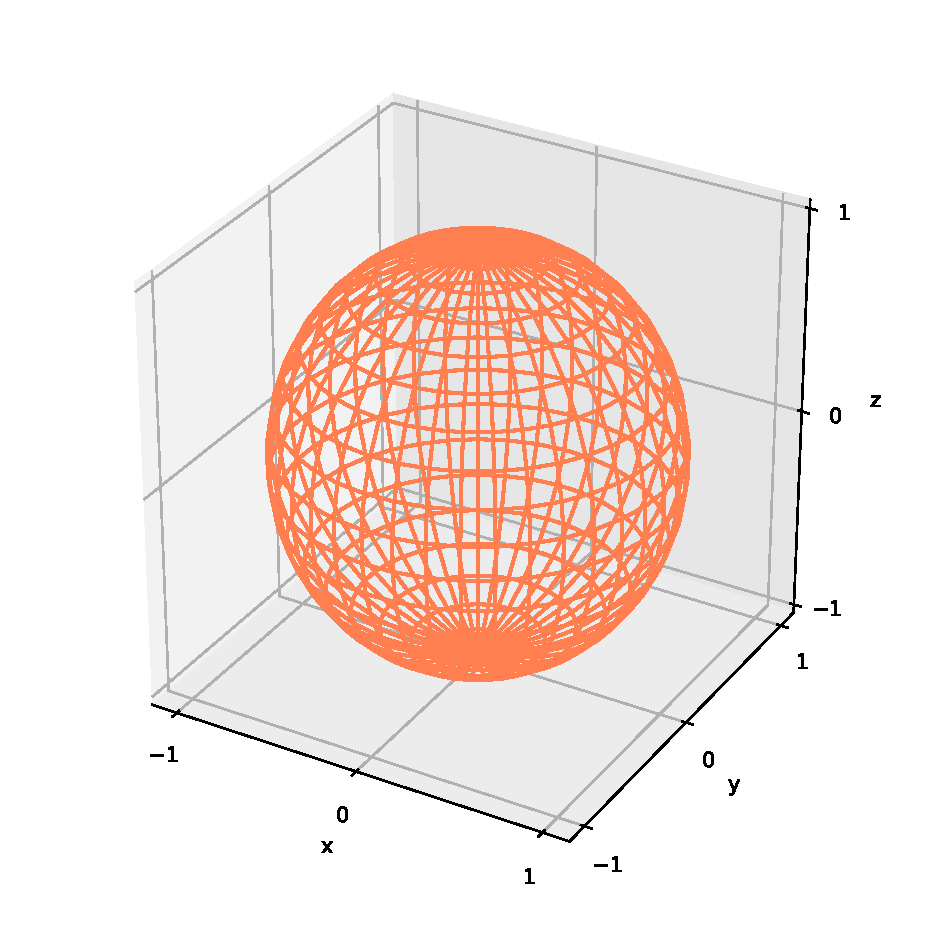
\epsfig{file=Sphere.eps}
\caption{Figure for Sphere}
\end{center}
\end{figure}

\end{document}

% LocalWords:  EGR 103L NetID Chapra OC 0c chapra py
